%%%%%%%%%%%%%%%%%%%%%%%%%%%%%%%%%%%%%%%%%%%%%%%%%%%%%%%%%%%%%%%%%%%%%%%%%%%%%%%%%%%%%%%%%
% Autor:        Torres Galicia Uriel
% Fecha:        26/08/2025
%%%%%%%%%%%%%%%%%%%%%%%%%%%%%%%%%%%%%%%%%%%%%%%%%%%%%%%%%%%%%%%%%%%%%%%%%%%%%%%%%%%%%%%%%

\documentclass[a4paper,11pt]{article}                 % Papel tamaño carta, texto de 11pt.
\usepackage[top=2.5cm, bottom=2cm, left=2.2cm, right=2.2cm]{geometry} % Margenes
\usepackage[T1]{fontenc}                              % Indicamos la codificación de las fuentes.
\usepackage[utf8x]{inputenc}                          % Definimos la codificación.
\usepackage{lmodern}                                  % Para poder usar acentos.
\usepackage[spanish]{babel}                           % Usaremos idioma español.
\usepackage{amsmath}                                  % Para formulas matemáticas.
\usepackage{graphicx}                                 % Para imágenes.
\usepackage{float}                                    % Para posicionar objetos.
\usepackage{booktabs}                                 % Para formatear tablas.
\usepackage{hyperref}                                 % Para enlaces y referencias.
\usepackage{listings}                                   % Para resaltar la sintaxis de 
\usepackage{listings} % Para resaltar la sintaxis de código
\usepackage{xcolor}   % Para usar colores

% Configuración del estilo para C++
\lstdefinestyle{cppstyle}{
    language=C++,                       % Lenguaje
    backgroundcolor=\color{white},      % Color de fondo
    basicstyle=\ttfamily\small,         % Estilo básico de la fuente
    keywordstyle=\color{blue},          % Color de las palabras clave
    commentstyle=\color{gray},         % Color de los comentarios
    stringstyle=\color{red},            % Color de las cadenas
    numbers=left,                       % Números de línea a la izquierda
    numberstyle=\tiny\color{gray},      % Estilo de los números de línea
    stepnumber=1,                       % Cada línea numerada
    numbersep=5pt,                      % Distancia de los números de línea
    showspaces=false,                   % No mostrar espacios
    showstringspaces=false,             % No mostrar espacios en cadenas
    showtabs=true,                      % Mostrar tabulaciones
    tabsize=2                    % Tamaño de tabulación
}



\def\logoUNAM{%
  \begin{picture}(0,0)\unitlength=1cm
    \put (-3.5,-3) {
\includegraphics[width=8em]{images/escudo-unam}}
  \end{picture}
}

\def\logoFI{%
  \begin{picture}(0,0)\unitlength=1cm
    \put (0.5,-3) {
\includegraphics[width=8em]{images/escudo-fi}}
  \end{picture}
}

%%%%%%%%%%%%%%%%%%%%%%%%%%%%%%%%%%%%%%%%%%%%%%%%%%%%%%%%%%%%%%%%%%%%%%%%%%%%%%%%%%%%%%%%%
\author{Torres Galicia Uriel}                                                         % Autor.
\title{Nombre del curso~\footnote{Aclaraciones}}                        % Titulo del curso.
\date{26/08/25)}                                                         % Fecha de entrega.

\def\universidad{Universidad Nacional Autónoma de México}               % Nombre de la universidad.
\def\facultad{Facultad de Ingeniería}                                   % Nombre de la facultad.
\def\semestre{2024-2}                                                   % Semestre lectivo.
\def\laboratorio{División de Ingeniería Eléctrica}                      % Nombre de la división.
\def\carrera{Ingeniería en computación}                                 % Nombre de la carrera.
\def\asignatura{Computación Gráfica e Interacción Humano Computadora}   % Nombre de la asignatura.
\makeatletter

%%%%%%%%%%%%%%%%%%%%%%%%%%%%%%%%%%%%%%%%%%%%%%%%%%%%%%%%%%%%%%%%%%%%%%%%%%%%%%%%%%%%%%%%%

\begin{document}
  % Titulo del documento con logos.
  \begin{center}
    \logoUNAM {\Large \universidad} \logoFI\par
    {\large \facultad}\par

    \laboratorio\par
    \carrera\par
    \asignatura
  \end{center}
  
  \vspace{2em} % Espacio adicional antes de la línea del encabezado
  \hrulefill\par

% Alineación a la derecha solo para el nombre del alumno
\begin{flushright}
    {\Huge \textbf{Introducción a OpenGL}} \\[1em] % Nombre de la práctica, grande y en negritas.
    %{\Large \textbf{Nombre del curso}} \\[1em] % Nombre del curso en un tamaño más pequeño
\end{flushright}

\vspace{4em} % Espacio adicional

% Alineación a la izquierda para el resto de la información
\begin{flushleft}
    {\Huge \textbf{xxxxxxx}} \\[1em] % Nombre del autor 
    {\Large \textbf{N° de cuenta: xxxxxx}} \\[1em]
    {\Large \textbf{Grupo de laboratorio: 12}} \\[1em]
    {\Large \textbf{Grupo de teoría: 1}} \\[1em]
    {\Large \textbf{Semestre: 2026-1}} \\[1em]
    {\Large \textbf{Fecha límite de entrega: 26/08/2025}} \\[1em]
\end{flushleft}

\vspace{20em} % Espacio adicional

\begin{flushright}
    {\Huge \textbf{Calificación: \_\_\_\_\_ }} \\[1em] % Calificación
\end{flushright}

\pagenumbering{gobble}                              % Oculta el numero de pagina.

\newpage  
\tableofcontents                                    % Crea el indice o tabla de contenido.


%%%%%%%%%%%%%%%%%%%%
\section{Introducción}
\href{https://github.com/ramen-root/CGIHC}{Aquí el respositorio de GitHub}.

A partir del código proporcionado se pide:
\begin{itemize}
    \item Crear cuatro puntos.
    \item Crear dos líneas verticales paralelas.
    \item Crear un triángulo con la hipotenusa hacia abajo y el ángulo recto arriba a la izquierda.
    \item Un cuadrado o rectángulo con fondo.
\end{itemize}

%%%%%%%%%%%%%%%%%%%%


\section{Objetivos}
En ésta práctica de laboratorio se explorará el uso de OpenGL para el dibujo de primitivas 2D; utilizando las bibliotecas GLFW y GLEW.

El objetivo principal es familiarizarnos con la creación de un entorno gráfico básico donde podamos renderizar formas simples, como triángulos y cuadrados, en la pantalla. A través de la práctica, aprenderemos a definir y gestionar los datos de los vértices y los índices que describen nuestras primitivas.

Al final de esta práctica, se tendrá una comprensión básica de cómo funciona OpenGL en la creación de gráficos 2D. Así, en proyectos y prácticas futuras podremos aplicar estos conocimientos para desarrollar geometrías más complejas hechas a partir de las primitivas.

El código proporcionado establece un contexto de OpenGL y crea una ventana donde se dibujarán las primitivas. Comenzamos inicializando GLFW y configurando las propiedades de la ventana, como su tamaño y compatibilidad con OpenGL. Posteriormente, se carga GLEW para acceder a las funciones de OpenGL, y se imprime información relevante sobre la versión y el proveedor del sistema gráfico. 


\section{Desarrollo}
\subsection{Primera parte: Cuatro puntos}
En ésta primer parte, se editaron dos porciones de código. Primero modificamos \textbf{unsigned int indices[]}, especificamente sus valores, debemos entender que en ésta parte se hace referencia a los vértices en el arreglo de vértices; es decir, el arreglo \textbf{indices}. El código queda de la siguiente forma:

% Bloque de código en C++
\begin{lstlisting}[style=cppstyle]
unsigned int indices[] = {
    3, 0, 1, 2 // Conecta 4 puntos en orden deseado
};
\end{lstlisting}

Ahora modificamos la función que dibuja los puntos, quedando de la siguiente forma:
% Bloque de código en C++
\begin{lstlisting}[style=cppstyle]
glPointSize(10);
glDrawArrays(GL_POINTS, 0, 4);
\end{lstlisting}

Modificamos el tamaño de los puntos (de 1 a 10) y después indicamos que usaremos cuatro vértices; con \textbf{GL\_POINTS} dibujamos los puntos, indicamos que queremos dibujar los cuatro puntos, cambiamos de \textbf{0,1} a \textbf{0,4}.


\subsection{Segunda parte: Dos líneas verticales paralelas}
Se toman nuevamente los índices del punto anterior, es decir.
% Bloque de código en C++
\begin{lstlisting}[style=cppstyle]
unsigned int indices[] = {
    3, 0, 1, 2 // Conecta 4 puntos en orden deseado
};
\end{lstlisting}

Ahora modificamos la función \textbf{glDrawArrays}, cambiándole el parámetro a \textbf{4} para indicar que tome los cuatro vértices nuevos. De la siguiente forma:
% Bloque de código en C++
\begin{lstlisting}[style=cppstyle]
glDrawArrays(GL_POINTS, 0, 4);
\end{lstlisting}

\subsection{Tercer parte: Triángulo}
Para dibujar el triángulo con la hipotenusa hacia abajo y el ángulo recto arriba a la izquierda, nuevamente se modifica \textbf{unsigned int indices[]}. En este caso agregamos tres vértices.
Podemos visualizarlo de la siguiente manera:

\begin{figure}[H] % 'h' indica que la figura debe colocarse aquí
    \centering % Centra la imagen
    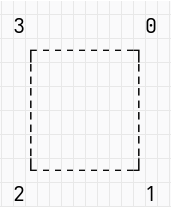
\includegraphics[width=0.2\textwidth]{images/img1.png} % Ajusta el ancho de la imagen
    \caption{Los índices estarían ubicados así} % Título de la figura
    \label{fig:indices} % Etiqueta para referenciar la figura
\end{figure}
Entonces para el triángulo deseado, usamos los índices 3,0,2. El código quedaría de la siguiente manera:
% Bloque de código en C++
\begin{lstlisting}[style=cppstyle]
unsigned int indices[] = {  // note that we start from 0!
    3,0,2,// second Triangle
    0,1,3,
};
\end{lstlisting}
No debemos olvidar invocar la función:
% Bloque de código en C++
\begin{lstlisting}[style=cppstyle]
glDrawElements(GL_TRIANGLES, 4,GL_UNSIGNED_INT,0);
\end{lstlisting}

\subsection{Cuarta parte: Rectángulo}
Aquí dibujamos simultaneamente dos triángulos, usando \textbf{glDrawArrays(GL\_TRIANGLES,0,3);} y \textbf{glDrawElements(GL\_TRIANGLES, 4,GL\_UNSIGNED\_INT,0);}. Usamos los índices anteriores, la idea es dibujar un triángulo rectángulo con la hipotenusa hacia abajo y el ángulo recto arriba a la izquierda y otro triángulo con la hipotenusa hacia arriba y el ángulo recto abajo a la izquierda; los triángulos deben estar pegados por la hipotenusa; así el espectador lo verá como un rectángulo.
Los índices son así:
% Bloque de código en C++
\begin{lstlisting}[style=cppstyle]
unsigned int indices[] = {  // note that we start from 0!
    3,0,2,// second Triangle
    0,1,3,
};

\end{lstlisting}
Se ejecutan ambas funciones a la vez:
% Bloque de código en C++
\begin{lstlisting}[style=cppstyle]
glDrawArrays(GL_TRIANGLES,0,3);
glDrawElements(GL_TRIANGLES, 4,GL_UNSIGNED_INT,0);
\end{lstlisting}

\section{Resultados}
\subsection{Primer parte: cuatro puntos}
\begin{figure}[H] % 'h' indica que la figura debe colocarse aquí
    \centering % Centra la imagen
    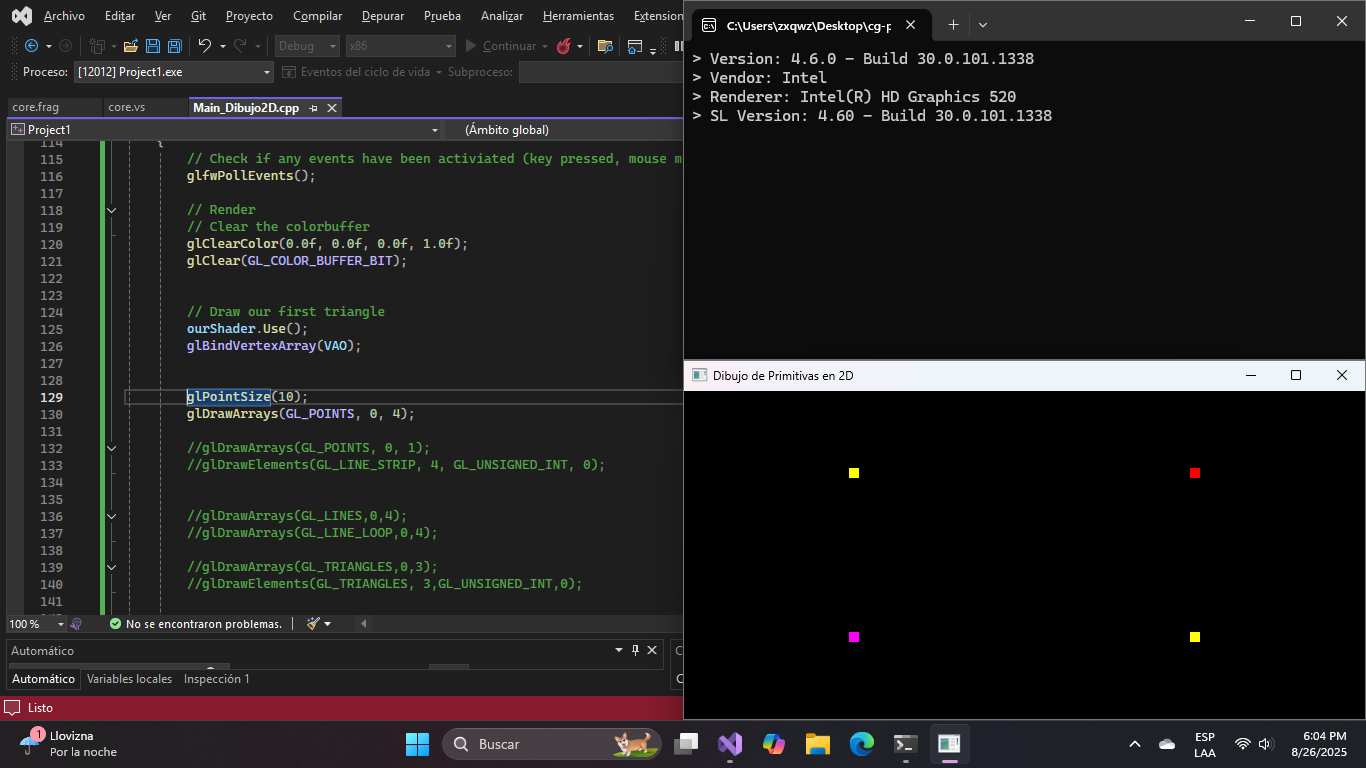
\includegraphics[width=0.6\textwidth]{images/dots.png} % Ajusta el ancho de la imagen
    \caption{Cuatro puntos} % Título de la figura
    \label{fig:dots} % Etiqueta para referenciar la figura
\end{figure}
\subsection{Segunda Parte: dos líneas}
\begin{figure}[H] % 'h' indica que la figura debe colocarse aquí
    \centering % Centra la imagen
    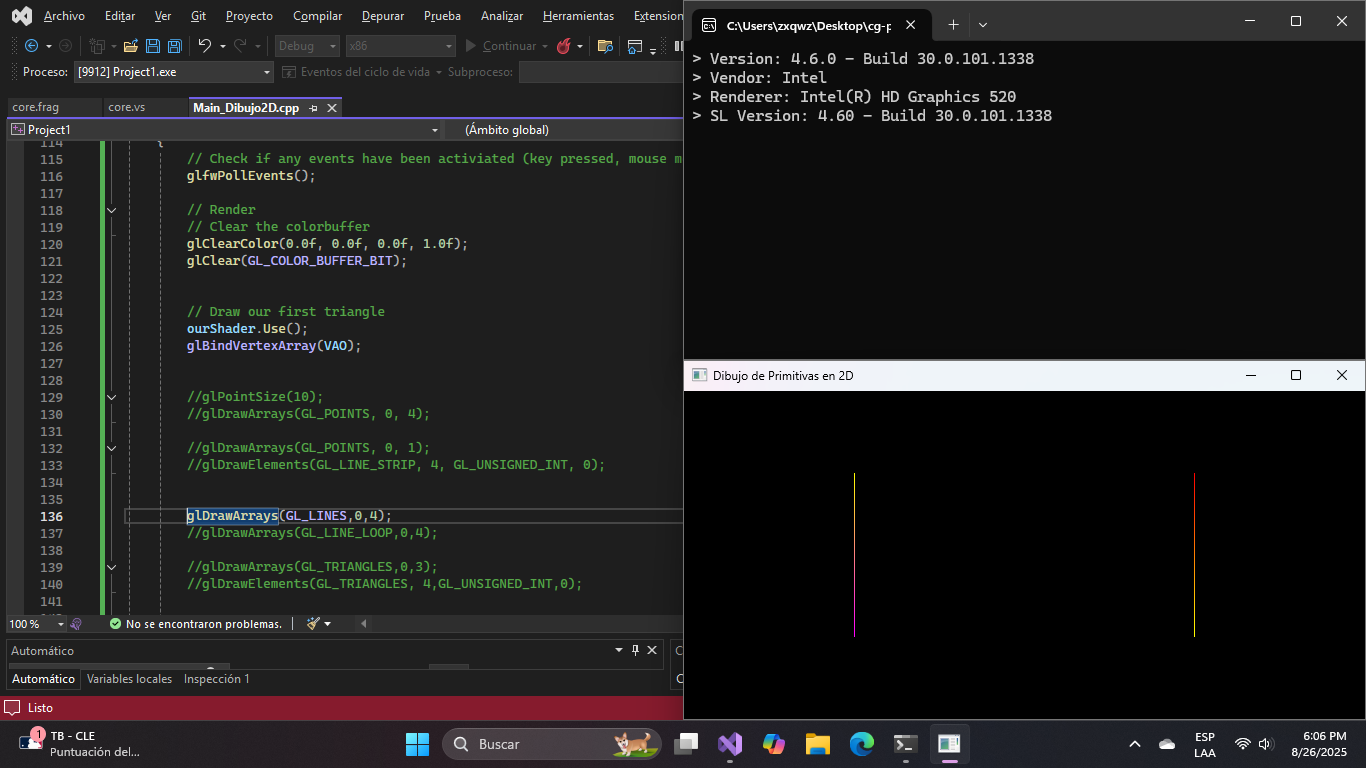
\includegraphics[width=0.6\textwidth]{images/lines.png} % Ajusta el ancho de la imagen
    \caption{Dos líneas verticales paralelas} % Título de la figura
    \label{fig:line} % Etiqueta para referenciar la figura
\end{figure}
\subsection{Tercer parte: triángulo}
\begin{figure}[H] % 'h' indica que la figura debe colocarse aquí
    \centering % Centra la imagen
    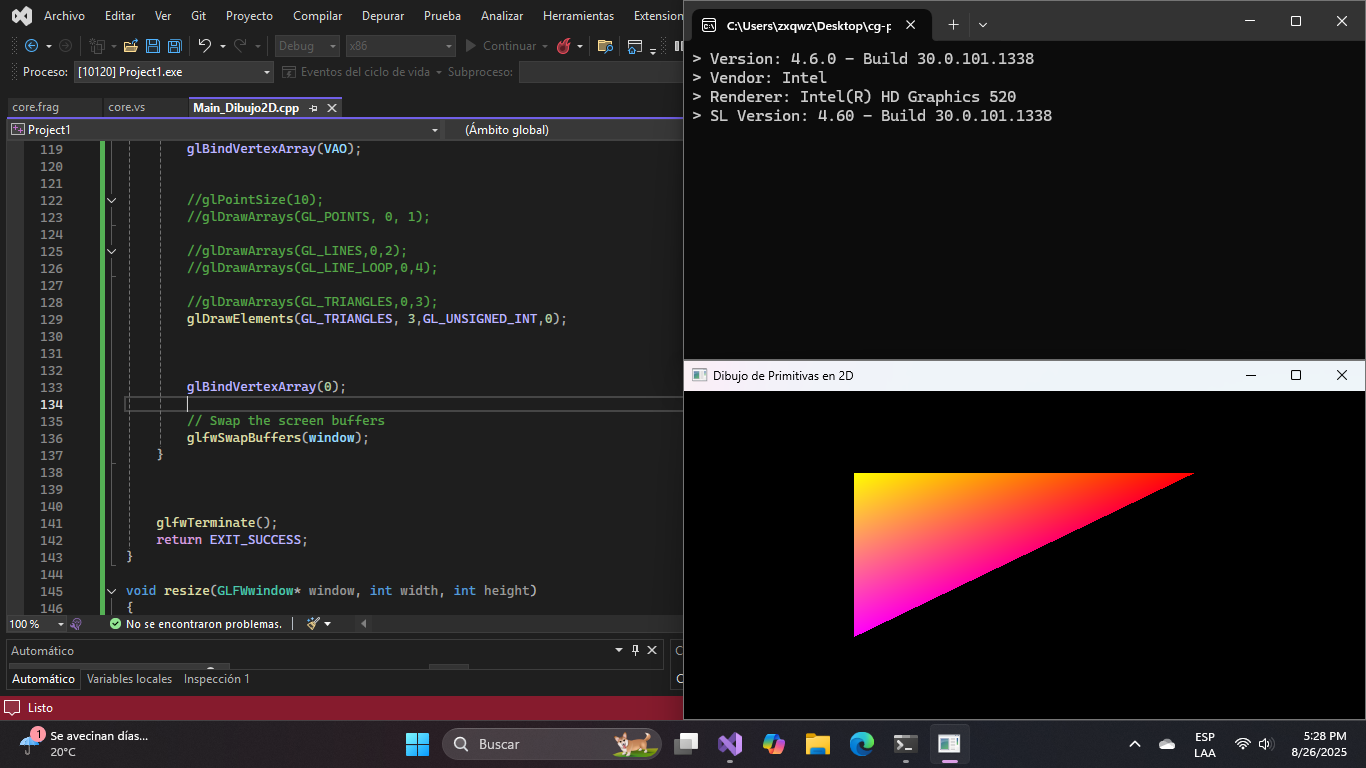
\includegraphics[width=0.6\textwidth]{images/triangle.png} % Ajusta el ancho de la imagen
    \caption{Triángulo con la hipotenusa hacia abajo y el ángulo recto arriba a la izquierda} % Título de la figura
    \label{fig:triangle} % Etiqueta para referenciar la figura
\end{figure}
\subsection{Cuarta parta: rectángulo}
\begin{figure}[H] % 'h' indica que la figura debe colocarse aquí
    \centering % Centra la imagen
    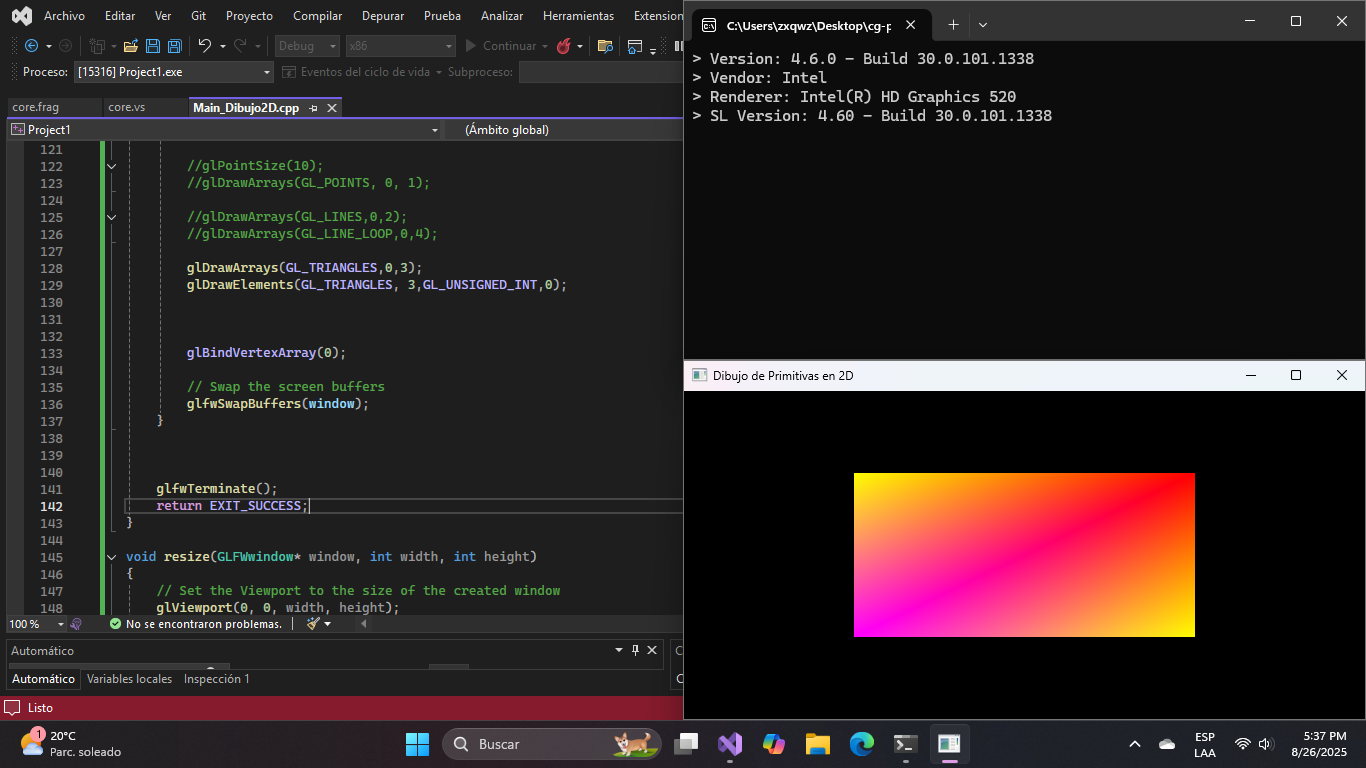
\includegraphics[width=0.6\textwidth]{images/square.png} % Ajusta el ancho de la imagen
    \caption{Rectángulo} % Título de la figura
    \label{fig:square} % Etiqueta para referenciar la figura
\end{figure}
\section{Conclusión}
\begin{itemize}
    \item Podemos definir una arreglo (en este caso \textbf{vertices}), para definir datos que se usarán para dibujar las primitivas gráficas; los primeros tres valores definen las coordenadas en el espacio 3D (x,y,z) y los últimos tres valores definen el color (RGB).
    \item En índices se define el órden en el que se deben dibujar los vértices; esto nos resulta útil a la hora de dibujar primitvas como triángulos o puntos sin tener que duplicar los datos de los vértices. 
    \item Cada número en el arreglo indices hace referencia a la posición de un vértice en el arreglo vertices. Por ejemplo, el primer triángulo se forma utilizando los vértices en las posiciones 3, 0 y 2 del arreglo vertices.
    \item glPointSize() establece el tamaño de los puntos.
    \item glDrawArrays(GL\_POINTS, 0, 4); - dibuja vértices como puntos, el primer parámetro GL\_POINTS indica que se deben dibujar puntos. El segundo parámetro 0 es el índice del primer vértice a dibujar, y el tercer parámetro 4 indica cuántos vértices se deben dibujar (en este caso, los primeros 4 vértices del arreglo vertices). 
    \item glDrawElements(GL\_LINE\_STRIP, 4, GL\_UNSIGNED\_INT, 0); - Este comando dibuja una línea que conecta los vértices en el orden especificado por el arreglo indices. GL\_LINE\_STRIP indica que se deben dibujar líneas conectando los vértices en secuencia. El segundo parámetro 4 indica cuántos índices se deben usar del arreglo indices, y GL\_UNSIGNED\_INT especifica el tipo de datos de los índices.
    \item glDrawArrays(GL\_LINE\_LOOP, 0, 4); - Este comando dibuja un bucle de líneas que conecta los vértices en el orden especificado, formando un polígono cerrado. En este caso, se conectan los primeros 4 vértices.
    \item glDrawArrays(GL\_TRIANGLES, 0, 3); - Este comando se utiliza para dibujar triángulos utilizando los vértices especificados en el arreglo vertices. GL\_TRIANGLES: Este parámetro indica que se deben dibujar triángulos. OpenGL tomará cada grupo de tres vértices consecutivos del arreglo de vértices y los conectará para formar un triángulo. 0: Este es el índice del primer vértice a utilizar. En este caso, comenzamos desde el primer vértice (índice 0). 3: Este parámetro indica cuántos vértices se deben utiliza1r para dibujar. En este caso, se utilizan los primeros 3 vértices del arreglo vertices.
    \item Se lograron resolver los tres ejercicios jugando con los índices y los argumentos de las funciones que dibujan las primitivas.
\end{itemize}


\vspace{1cm}
\noindent\textbf{Referencias}
\newline
No hay bibliografía propiamente, pero sin esto no podría haber resuelto los ejercicios:
\begin{itemize}
    \item AxDTb1IaDpA. (2021). \textit{OpenGL Como instalar definitivamente}. YouTube. Recuperado de \url{https://www.youtube.com/watch?v=AxDTb1IaDpA}
    \item Intel. (n.d.). \textit{Intel 7th-10th Gen Processor Graphics Windows}. Recuperado de \url{https://www.intel.com/content/www/us/en/download/776137/intel-7th-10th-gen-processor-graphics-windows.html}
\end{itemize}

\end{document}